\documentclass{SeminarV2}

\usepackage[latin1]{inputenc}
\usepackage{amssymb,amsmath,array}
\usepackage{graphicx}
\usepackage{placeins}

\usepackage{fancyvrb}
\fvset{tabsize=4}

\usepackage[]{hyperref}
\usepackage{framed}


\usepackage{listings,color}

\definecolor{verbgray}{gray}{0.9}

\lstnewenvironment{code}{%
    \lstset{backgroundcolor=\color{verbgray},
        frame=single,
        basicstyle=\small \ttfamily,
        framerule=0pt,
        breaklines=true
        }}{}

%\lstset{%
%	language=[LaTeX]TeX,
%	basicstyle=\ttfamily,
%	breaklines=true,
%	columns=fullflexible,
%    showtabs,
%    showstringspaces=true
%}

\newcommand{\shellcmd}[1]{\smallskip\\\indent\indent\texttt{\footnotesize\$ #1}\par\vspace{5pt}}

\newcommand{\mV}{ \texttt{multiVitamin} }


%
\voffset -2 cm \hoffset -2 cm \addtolength{\textwidth}{3cm}
\addtolength{\textheight}{2cm}\addtolength{\leftmargin}{0cm}



\begin{document}
%style file for Seminar manuscripts
\title{
    \vspace{7cm}
    
    {\Huge multiVitamin}
    
    In-terminal multiple graph alignment tool
    
    \vspace{2cm}
    
    User Manual
    
    \vspace{8cm}
}

%***********************************************************************
% AUTHORS INFORMATION AREA
%***********************************************************************
\author{Clemens Malkawi$^1$, Michel Kreck�$^1$, Maximilian Joas$^1$
%
% Optional short acknowledgment: remove next line if non-needed
%\thanks{This is an optional funding source acknowledgement.}
%
% DO NOT MODIFY THE FOLLOWING '\vspace' ARGUMENT
\vspace{.3cm}\\
%
% Addresses and institutions (remove "1- " in case of a single institution)
University of Leipzig  - Department of Computer Science \\
Augustusplatz 10, 04109 Leipzig  - Germany\\}

%
% Remove the next three lines in case of a single institution

%***********************************************************************
% END OF AUTHORS INFORMATION AREA
%***********************************************************************

\maketitle

\newpage
\tableofcontents

\newpage
\section{multiVitamin}
\mV is a software package which allows users to perform multiple alignments with graphs.
There are two algorithms available for this task. The Bron Kerbosch (BK) \cite{bron1973algorithm}
and the algorithm originally published by Cordella et al. (VF2) \cite{sansone2001improved}. Details on the algorithms can be found in the
theory section.\\
The main function of the package is to align two or more graphs following a binary alignment guide tree containing the "best" alignment procedure. The resulting multiple graph alignment is represented as one single graph itself. Next to this main function, there is also the possibility to show all co-optimals of an alignment between 2 graphs or to view graphical representations of graphs.  
Sounds exciting, so let's get started!

\section{Installation}

Clone the repo from github to [yourDir] with 
\shellcmd{git clone https://github.com/mk36fyvy/multivitamin.git}
Navigate to the directory containing the setup.py file 
\shellcmd{cd [yourDir]/multivitamin/multivitamin}
and type
\shellcmd{pip3 install -e .}
Done, now you can run \mV in the command shell. You can test if the installation was successful by typing
\shellcmd{multiVitamin -h}



\section{Graph Format}

A good first step is to familiarize yourself with the graph format. A graph file is basically a text file, we use the extension '.graph'. It is also used interiorly to identify graph files as such.

The file itself is structured as follows (see below for an example): \\

Every graph consists of nodes and edges. Every node has an id, which is a unique integer (handled as a String internally) for each node. Optionally, nodes can be labelled. The id and label are separated by a semicolon (\texttt{;}) in the '.graph'-file. The edges are two connected nodes and represented by the ids of the two nodes separated by a semicolon.\\

Now, let's walk through the overall structure of the '.graph'-file: 

\begin{itemize}
	\item There is a possibility to insert comment lines by preceding comments with \texttt{//} or writing \texttt{;comment} after the comment. These lines will be ignored by the parser. They can be written anywhere in the first paragraph.
	\item The first line indicates the author of the graph. This line has to start with the word "author" to be recognized by the parser.
	\item The second and third lines show the number of nodes and edges respectively. The parser only sees two consecutive integers at the end of the lines, so it is important that the number of nodes is provided before the number of edges.
	\item The next three lines are booleans that indicate whether the nodes / edges are labelled and if the graph is directed. It is important to stick to the order indicated in the \hyperref[fig:graph_example]{example} below.
	\item The blank line indicates the start of the node section. It is important to choose an integer as node id. The label can contain any symbol, except for \texttt{;}.
	\item The node section is separated from the edge section again by a blank line. If the \texttt{Directed graph} option is set to \texttt{False}, the edges are considered undirected. Internally, every edge's reverse is then added to the graph.  
\end{itemize}

\noindent
Let's look at a small example graph for illustration. The graph has 6 nodes which are all labelled with a 'c' and 6 edges which are not labelled. Your graphs need to have exactly this format to use this package. Especially the blank lines are important. You can find a decent number of further examples at \texttt{multivitamin/graph\_examples}. Now that you are familiar with the graph format, we can take a look at how to use the package.


\begin{framed}
\begin{verbatim} 
//this is a sample graph
AUTHOR: Michel K.
#nodes;6
#edges;6
Nodes labelled;True
Edges labelled;False
Directed graph;False

1;c
2;c
3;c
4;c
5;c
6;c

1;2
1;6
2;3
3;4
4;5
5;6
\end{verbatim}
\end{framed}


\newpage
\section{Multiple graph alignment}
\subsection{Graph alignment with BK algorithm}
Consider the basic use without any optional flags for the start. You do not have to be in the directory of the package to use \mV. To get an overview of all the flags you can type
\shellcmd{multiVitamin -h}

If you are experienced with command-line tools the information provided by this command might be sufficient to get you started.\\


\begin{figure}[h!]
\begin{code}
usage: multiVitamin [ -h | -m | -c | -v | -d ] [-a] [-s] [-t] [-g]
for example: multiVitamin -ga VF2 -m g1.graph g2.graph g3.graph

multiVitamin - A multiple alignment tool for graphs

Required arguments (These arguments are mutually exclusive):

-h, --help                  show this help message and exit
-m, --multiple <files...>   provide .graph files for multiple alignment '.' 
                              takes all .graph files in the directory as 
                              arguments
-c, --coopt <files...>      provide 2 graphs which will be aligned.
                              Co-optimals will be saved in ./results
-v, --view <files...>       get a visual representation of the given graphs 
                              in one window. This can get confusing for 
                              large or many graphs. Use -d if you want to 
                              see one window per graph.
-d, --disp-mult <files...>  get a visual representation of the given graphs 
                              in one window per graph.

Optional arguments:

-a, --algorithm <BK|VF2>    indicate an alignment-algorithm (default: BK)
                              Warning: VF2 is only suited if there is true 
                              graph-subgraph isomorphism!
-s, --save-all              save all the graphs produced during the 
                              alignment. The graphs are saved as 
                              "[newick].graph"
-t, --save-shorter          save an additional version of the alignment 
                              graph with much shorter node ids
-g, --save-guide            save the guide tree in Newick-format as 
                              "newick.txt"

\end{code}
\end{figure}


There are three main functions resulting in four mutually exclusive flags. One of them is always required to make multiVitamin work. For starters, we look at the case of a multiple alignment of graphs, which is considered the standard use case. 

Just type:
\shellcmd{mulitVitamin -m <pathToGraphFile1.graph> <pathToGraphFile2.graph> ...}
  
This aligns the given graphs with the default algorithm, which is BK. The resulting terminal output provides all the important information about the alignment. An example output can be found below. 

\label{title:multid}
In order to assure the uniqueness of node's IDs in a multiple alignment, every node owns a \texttt{mult\_id} attribute, which comes into play here. First, every graph gets a \textit{unique abbreviation string}. It is built from the first two letters of the graph file name and an index, which is incremented each time, a two letter combination is already taken for the specific multiple alignment. 

%Reading graph1.graph from Clemens M., Max. J, Michel K.
%Successfully parsed graph1.graph
%
%Reading graph2.graph from Clemens M., Max. J, Michel K.
%Successfully parsed graph2.graph
%
%
%                 _ _   _       _  _                   _       
%                | | | (_)     (_)| |                 (_)      
% _ __ ___  _   _| | |_ \ \   / / | |_  __ _ _ __ ___  _ _ __  
%| '_ ` _ \| | | | | __| \ \ / / ||  _|/ _` | '_ ` _ \| | '_ \ 
%| | | | | | |_| | | |_| |\ V /| || |_| (_| | | | | | | | | | |
%|_| |_| |_|\__,_|_|\__|_| \_/ |_| \__|\__,_|_| |_| |_|_|_| |_|
%
%                                                v1.0.0      
%
%Calculating multiple alignment with BK algorithm...

\begin{figure}[h!]
    \begin{code}
        
        *****************************************************************
        *                                                               *
        *                          RESULTS                              *
        *                                                               *
        *****************************************************************
        
        ---GRAPH ABBREVIATIONS--------------
        
        gr1	>>	graph1
        gr2	>>	graph2
        
        
        ---ALIGNMENT------------------------
        
        *NODES (ID, LABEL, NEIGHBOURS)
        gr1:4.gr2:2   'd'   ( gr1:1.gr2:5, gr1:2.gr2:3, gr1:5.gr2:4 )
        gr1:1.gr2:5   'a'   ( gr1:2.gr2:3, gr1:5.gr2:4, gr1:4.gr2:2, gr1:3.gr2:6 )
        gr1:2.gr2:3   'b'   ( gr1:1.gr2:5, gr1:5.gr2:4, gr1:4.gr2:2, gr1:3.gr2:6 )
        gr1:3.gr2:6   'c'   ( gr1:1.gr2:5, gr1:2.gr2:3 )
        gr1:5.gr2:4   'e'   ( gr1:1.gr2:5, gr1:2.gr2:3, gr1:4.gr2:2 )
        
        *EDGES (ID, LABEL)
        ( gr1:2.gr2:3,   gr1:3.gr2:6 )   ''
        ( gr1:4.gr2:2,   gr1:2.gr2:3 )   ''
        ( gr1:1.gr2:5,   gr1:3.gr2:6 )   ''
        ( gr1:1.gr2:5,   gr1:2.gr2:3 )   ''
        ( gr1:4.gr2:2,   gr1:1.gr2:5 )   ''
        ( gr1:4.gr2:2,   gr1:5.gr2:4 )   ''
        ( gr1:1.gr2:5,   gr1:5.gr2:4 )   ''
        ( gr1:2.gr2:3,   gr1:5.gr2:4 )   ''
        
        
        ---NEWICK TREE----------------------
        
        (graph1,graph2)
        
        ********************************************************************
        
        Successfully created the directory /home/micheltower/Documents/multivitamin_project/multivitamin/graph_examples/other/results
        All files will be saved here.
        Saved graph as gr1-gr2.graph
        
        Saved graph id abbreviations as graph_abbreviations.txt
        
    \end{code}
\end{figure}

In the example, graphs 1 and 2 are called gr1 and gr2 respectively. This abbreviation is used to build the unique node \texttt{mult\_id}s.\\\par

\noindent
Let's look at the first line depicting a node in the nodes section:  

\begin{code}
gr1:4.gr2:2   'd'   ( gr1:1.gr2:5, gr1:2.gr2:3, gr1:5.gr2:4 )
\end{code}

The node \texttt{gr1:4.gr2:2} originates from the alignment of \textbf{node 4 from graph1} and \textbf{node 2 from graph2}. Note that there is a '\texttt{:}' between the graph and the corresponding original node ID and a '\texttt{.}' between the nodes of different graphs. 

As indicated in the terminal output, what follows written between ' ' is the label of the node. The label handling during alignment with BK algorithm is specified in 
\\\par\indent\texttt{[yourDir]/]multivitamin/multivitamin/utils/modular\_product.py}\\\par

\noindent
At the moment, if any semantic label checks are needed, you should use the VF2 algorithm. See \hyperref[title:VF2]{below} for more information.

The neighbours of the node are indicated in parentheses, again indicated by the notation explained above.

The edges section shows the edges as follows: \texttt{node1} and \texttt{node2} are indicated by their \texttt{mult\_id} followed by their label. 

The last section indicates the alignment guide tree in conventional Newick format. \\\par

Naturally, apart from the terminal output, \mV saves the results from the alignment in actual files as well. Every generated file will be saved in the \texttt{./results} folder, with '.' being your current working directory. If the folder is already present, \mV simply adds the files, if not, it creates the directory automatically.\\\par

\noindent
Files that will be created after successful multiple alignment:

\bigskip
\begin{tabular}{rp{0.65\textwidth}}
    \textbf{graph\_abbreviations.txt} & easily parseable text file which indicates the full name and abbreviation couples of the graphs used in the alignment\\\\
    \textbf{$<$g1-g2-...$>$.graph} & the graph resulting from the alignment (in .graph-format). The file contains a comment line indicating the guide tree by which it was obtained\\
\end{tabular}
\bigskip

\noindent
More files can be created by using optional flags. These are summarized \hyperref[title:Optional flags]{below}.



\subsection{Graph alignment with VF2 algorithm}
\label{title:VF2}
Let us still consider the basic use case with the required flag \texttt{-m}. This flag can be combined with all optional flags (see \hyperref[title:Optional flags]{below}). \texttt{-a} lets you choose between BK and VF2 algorithm. In order to use the VF2 algorithm for the alignment simply type
\shellcmd{multiVitamin -a VF2 -m <pathToGraphFile1.graph> <pathToGraphFile2.graph> ...}

Please note, that VF2 algorithm is only suited for graph-subgraph isomorphism, or else the alignment will fail. Broadly speaking, the smaller graph must always fit entirely into the bigger graph. Hence, every node in the smaller graph must have a corresponding node in the bigger graph. The edges must be alignable in an analogous way. 

Despite this restriction, VF2 is still a powerful algorithm. Apart from having overall faster performance than BK algorithm\cite{bron1973algorithm}, you have the possibility to set semantic restrictions for the alignment. This means that you can forbid alignment of structurally similar nodes by setting conditions on the compatibility of their label.

These conditions can be set in the \texttt{custom.py} file. 

\subsubsection{Custom.py}
The \texttt{custom.py} file can be found in the multivitamin directory of the root folder, the same directory as \texttt{setup.py}. This file contains the function \texttt{check\_semantics} function, which by default always returns true. The code of the \texttt{custom.py} file looks as follows:

\begin{code}
def check_semantics( n, m ):
    '''This function is used in VF2 algorithm to decide,
    whether aligning to nodes is allowed from the
    label point of view.
    In the sample example below, two nodes will only
    be accepted as a legal matching, if the two
    labels are exactly the same.

    Insert your scoring logic below:'''

#    if n.label == m.label:
#        return True
#    else:
#        return False

    return True

def get_results_dir():
    '''define, where the result files will be saved.
    Default is a dir named 'results' in the current
    working directory'''

    return "/results"
\end{code}

As mentioned, returns true per default. This means, that there are no label restrictions for alignment. If a simple label equality restriction is desired, simply uncomment the four lines and comment out the default \texttt{return True}. This results in nodes only being aligned, if their label is exactly the same. However, you can go as crazy as you want with this method.

Additionally, you can specify the path where your results should be saved (relative from your current working directory). Simply replace \texttt{"/results"} by any valid string value. 

Before we jump right to the implemented basic classes, which you might want to use for a highly sophisticated \texttt{check\_semantics} function, we
want to take a look at the optional flags.
Note: A change in the basic classes is generally not recommended.

\newpage
\subsection{Optional flags}
\label{title:Optional flags}
Apart from the flag -a which allows to specify the algorithm used for the alignment, there are some more optional flags, which can be used to let \mV save a couple more useful files at the end of the alignment. All of these files will be saved in the \texttt{results/} directory mentioned above.

\noindent
Files that can optionally be created by using flags:

\bigskip
\begin{tabular}{rp{0.9\textwidth}}
    \textbf{-s}  & Saves all intermediate graphs that were produced along the alignment guide tree. Normally you would only get the final alignment graph out of the alignment. However, in some cases, it might be useful to get all the graphs produced in the alignment.\\\\
    \textbf{-t}  & Saves a version of the alignment graph with much shorter node ids. Even though this makes it impossible to get information about which nodes originated from which ones in the original graphs, it might be a good idea to use this graph for further alignment to assure, that the node IDs stay readable and unique.\\\\
    \textbf{-g}  & Saves the alignment guide tree in an easily parseable way as '\texttt{newick.txt}'\\
\end{tabular}
\bigskip


\section{Additional features}
In order to make \mV work, you need one (exactly one) of the following flags: \texttt{-m, -c, -v, -d}. The \texttt{-m} option has been discussed in depth in the previous sections. It can be used with every optional flag.

In addition to multiple graph alignment, \mV presents two more features which will be presented in the following sections.


\subsection{Getting alignment co-optimals}
The \texttt{-c} flag works with exactly two input files. It gives all the co-optimal alignments of the two given graphs. You can run it like so
\shellcmd{multiVitamin -c <pathToGraphFile1.graph> <pathToGraphFile2.graph>}
In many cases, when two graphs are aligned, there are multiple different, yet optimal ways of doing so; optimal meaning with equal maximal amount of nodes in the alignment. The -c flag calculates and saves all these alignment graphs. Note that only \texttt{-a} (algorithm choice) is a valid optional flag for this feature.


\subsection{Viewing graphs}
The \texttt{-v} and \texttt{-d} flags offer access to graphical representations of \texttt{.graph} files. You can either provide one or more graphs with the flag like so
\shellcmd{multiVitamin -v <pathToGraphFile1.graph> ...}
The \texttt{-d} flag is used analogously. Nodes are represented as blue dots containing their ID followed by their label in \texttt{' '}, interconnected by lines which represent the edges in the graph. Naturally, no optional flag is compatible with this feature.

The two flags differ in behaviour if more than one \texttt{.graph} file is provided:
\begin{itemize}
    \item \texttt{-v} shows the graphs in one file with the different graph representations ordered in a window grid.
    \item \texttt{-d} shows every provided graph in a separate window. 
\end{itemize}



\section{Basic Classes}
    In order to represent our graph objects internally, we used three basic classes: a node class, an edge class and a graph class. As we think it might be helpful to know about our exact implementation of the graph objects in order to understand some errors you may encounter, we will give a brief overview of the base classes. 
    
    All classes have built-in print methods for more readable output as well as custom built-in  methods to compare objects of the same class. 
    
    Fig.\ref{fig:UML} shows a simple UML class diagram of our base classes. The most important methods and attributes will be explained below.\\ \bigskip \\

\begin{figure}[h!]
    %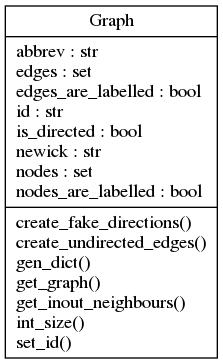
\includegraphics[width=0.5\textwidth]{classes.png}
    %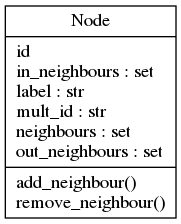
\includegraphics[width=0.5\textwidth]{node.png}
    %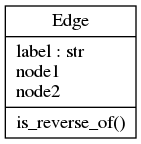
\includegraphics[width=0.5\textwidth]{edge.png}
    {\centering
	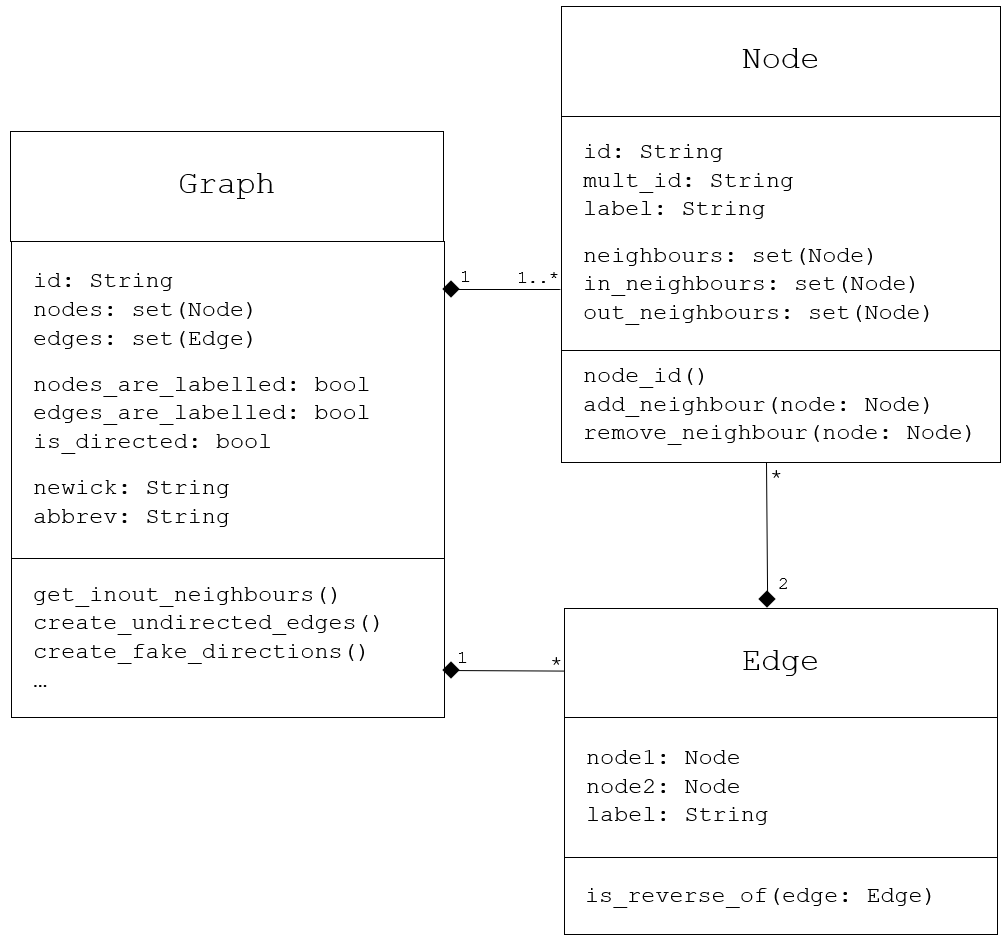
\includegraphics[scale=1.7]{multivitamin_basic_uml.png}
    }
    \caption{A UML class diagram of the base classes}
    \label{fig:UML}
\end{figure}


\subsection{Node class}
    The \texttt{Node} objects are seen in the context of a graph. Thus, every node contains information about its neighbours. Therefore a node has a \texttt{neighbours} attribute which is a set of \texttt{Node} objects. In case of directed graphs one can distingush between in and out neighbours, which is used internally in the VF2 algorithm. The \texttt{mult\_id} attribute gives an option to uniquely name the node in a mulitple alignment, as we already explained above.
    
    The \texttt{node\_id} method used internally to identify the node at many places simply returns the \texttt{mult\_id} attribute if it is not an empty String. Else, it returns the \texttt{id} attribute of the node.


\subsection{Edge class}
    An \texttt{Edge} object consists of two \texttt{Node} objects and an optional label. For each Edge it can be checked if it is the reverse of another edge. This only makes sense for directed graphs, because, as we already pointed out, undirected graphs are treated internally as having both one edge and its reverse respectively.


\subsection{Graph class}
    Besides the obvious attributes of nodes, edges and an id, a \texttt{Graph} object also has an \texttt{abbrev} attribute which was explained above. Since VF2 only works with directed graphs, we allowed our undirected graphs the to be treated as a directed graph internally. 
    
    Let us explain the most important methods of the \texttt{Graph} class.
    
    \begin{itemize}
        \item Consider edge A-B in the undirected graph G, A and B being nodes in G. \\The \texttt{create\_fake\_directions} method creates a new \texttt{Edge} object B-A to the already existing edge and adds it to G. 
    
        \item The method \texttt{create\_undirected\_edges} fills the \texttt{edges} set of the graph with the help of the \texttt{neighbours} sets of their nodes. 
    
        \item The method \texttt{get\_inout\_neighbours} fills the sets \texttt{in\_neighbours} and \texttt{out\_neighbours} of the \texttt{Node} objects in the graph's \texttt{nodes} set
    \end{itemize}


\section{Theoretical background of the algorithms}

\subsection{Bron Kerbosch algorithm}
The Bron Kerbosch algorithm indirectly solves the problem of finding a maximal common induced subgraph of two graphs G and H. This is done by finding the maximal clique in the modular product of G and H. The set of nodes of the modular product of G and H  is the cartesian product N(G)xN(H), with N being the set of all nodes of the corresponding graph. Any nodes (u,v) and (x,y), with u,x\,$\in$\,G and v,y\,$\in$\,H in the modular product are adjacent iff:

\begin{itemize}
	\item u and x were neighbours in G and y and x were neighbours in H
	\item u and x were not neighbours in G and y and v were not neighbours in H
\end{itemize}

Before using BK algorithm, we need to build the modular product of two graphs we want to align. Our implementation of BK (with pivot) is shown in the following code snippet.

\begin{figure}[h!]
\begin{code}
def bk_pivot ( self, r, p, x ):
	if not any ( [p, x] ):
		self.results.append(r)
		return r
	pivot = self.find_max_pivot( p, x )
	for v in p[:]:
		if  v in pivot.neighbours:
			continue
		r_ = r | {v}
		x_ = x & v.neighbours
		p_ = [n for n in v.neighbours if n in p ]
		self.bk_pivot ( r_, p_, x_ )
		p.remove(v)
		x.add(v)
\end{code}
\end{figure}

\newpage
The goal of BK is, as mentioned, to find the maximal clique in the modular product. A clique is a subgraph where every node is connected to every other node in the subgraph (=complete graph). A maximal clique is a clique so that no node can be added to the subgraph such that the subgraph remains complete.

The data structures are a list p, which is the list of candidates that could extend a clique, and the sets r and x. r contains all the nodes in a maximal clique and x is a set for blacklisting nodes. Blacklisting is used to not find the same cliques over and over again. Thus, x and p are only empty iff a new clique is found. \\\par

\noindent
Let us consider the case without pivoting first.
At the beginning, r and x are empty sets and p contains all the nodes of the modular product of the two input graphs. Then select one node v in p and check if it is part of a clique. The basic idea is to look at all the neighbours of this node, because these are the only nodes that can build a clique with n. 

At the very beginning, our new p\_ consists of all the neighbours from n, since p was empty at the beginning. In the first recursion step we select one of those neighbours, e.g nodes in our new p. Let us call it v\_. By default, we know that all these nodes in p\_ are neighbours of v. Now we intersect all the neighbours of v\_ with p. In that way, we get a new set of candidates. Every node in this set must be neighbour of v as well as v\_. 

This computation is repeated recursively until the candidate list p is empty. If our blacklisting set x is also empty, we found a clique. Of course, some bookkeeping of which nodes are in the clique has to be done. Therefore we add every node that we have contemplated to our result set r. When one recursive step finishes, we remove the node we used in the iteration from the candiates p and add it to the blacklist set x. This recursive process is then repeated for the next node in our candidate set.\\\par

\noindent
A short note on pivoting:
The pivoting is solely a performance optimization. It makes the recursion tree first deep and computes the wideness later. There are several ways to choose a pivot, it can be chosen at random or, as we did, by maximizing the intersection of the neighbours of the currently relevant node v and the union of p and x.

\subsubsection{BK in multiple alignment context}
BK only finds cliques in the modular product of two graphs. In a multiple alignment setting however, we would like to get a graph out of the clique, so we can use it for further alignment. To get a graph which one can work with out of the clique we need to delete the neighbours from the nodes, that are not in the subgraph anymore.

\subsection{VF2 algorithm}
As already mentioned, VF2 is an algorithm suited to finding graph isomorphism and graph-subgraph isomorphism. The inventors of the algorithms claim it to be highly memory efficient due to clever exploitation of the search space (depth-first). Since the theoretical foundations can be found in great detail in Cordella et al. \cite{sansone2001improved}, we will focus on the specific details of our implementation.

The algorithm takes two graphs as an input and outputs the mapping of the two graphs.

In order to understand the algorithm we need to explain some of the structures we use in the code (Python). We use two dictionaries (one for each graph) to store the mapping. The dictionary for graph 1 contains the nodes of graph 1 as keys. Their value becomes the nodes they map on in graph 2 as the mapping progresses (vice versa for graph 2). In our implementation, these dictionaries are called \texttt{core\_l} and \texttt{cores\_s} (s for small, l for large; if both graphs have the same size, the graph parsed first is referred to as the large one). If a node has not been mapped, the value of this node in the dictionary is a null node (e.g. a \texttt{Node} object with ID '-1' and empty label '').

 In order to find candidate pairs we implemented terminal sets. The current terminal sets of contain all nodes that are connected to nodes in the current mapping but are not yet in the mapping themselves. In praxis we have not only one terminal set per graph, but two because we distinguish between in and out neighbours. So we have four terminal sets in sum: \texttt{t\_in\_l} (terminal set for in-neighbours of the large graph), \texttt{t\_out\_l}, \texttt{t\_in\_s}, \texttt{t\_out\_s}. 
 
 The term 'set' might be misleading in our implementation, because we used dictionaries for storing which node is in which terminal set in at which depth. All nodes of each graph are keys and the recursion depth in which a node was added to a terminal set as value. The default value is 0, which means the node was not yet added to a terminal set. 
 
 Additionally, we use a helper dictionary that stores how many nodes are actually in the terminal sets at a given state. 
 
 Since the terminal sets and the \texttt{core\_s} and \texttt{core\_l} structures are shared across all recursion steps a state refers to the content of these structures in function of the current mapping and the currently contemplated pair of nodes, which are mapped on each other. Now you that you have achieved basic understanding of the data structures we look at the actual algorithm:\\\medskip\\
 
\begin{figure}[h!]
\begin{code}

def match(self, last_mapped=(Node("-1", ""), Node("-1", "")), depth=0):

    if self.s_in_small_g():
        self.append_result_graph( self.core_s )
        self.restore_ds( last_mapped[0], last_mapped[1], depth )
        return
    
    td = self.set_inout(last_mapped[0], last_mapped[1], depth)
    p = self.compute_p(td)
    
    for tup in p:
    
        if self.is_feasible(tup[0], tup[1], depth, td):
            self.compute_s_(tup[0], tup[1])
            self.match(tup, depth+1)
    
    self.restore_ds(last_mapped[0], last_mapped[1], depth)

\end{code}
\end{figure}

This is actual Python code from our implementation. Let us look at it line after line. 

\begin{itemize}
\item The \texttt{match} function takes the two nodes that got mapped to each other as input as well as the recursion depth. The default values are the null nodes and 0 for the depth. 

\item If every node of the smaller graph is mapped to a node of the larger graph, the algorithm found a valid graph-subgraph-isomorphism and saves the mapping in a \texttt{results} list. 

\item Else, VF2 counts how many nodes are in the terminal sets in the \texttt{set\_in\_out}. (Iterates through all the neighbours of the last mapped nodes and checks if these neighbours are in a terminal set)  The added nodes get the current recursion depth in the terminal dictionaries. 

\item Next, it is counted how many nodes are in the terminal sets. These counts are saved for every terminal set in the dictionary \texttt{td}. We need this information for the next step.

\item \texttt{compute\_p} returns a list of tuples. The tuples contain a node from each graph. The tuples are possible candidates to be mapped to each other. This list p is generated as follows: If both out terminal sets are not empty, the cartesian product is built out of the out terminal set of the large graph with the largest node of the out terminal set of the small graph. The equivalent happens for the in terminal sets if they are both not empty and the out terminal set are both empty. In case that all four terminal sets are empty, the cartesian product is built out of all the nodes that are not in the mapping of the large graph with the largest node that is not mapped in the small graph.

\item Next, VF2 iterates over this list and checks for the nodes in the tuple if it is feasible to map them to each other. There need to be two conditions met for that. Consider the process with one n node of the tuple (n,m) (the process is done analogously for the other node m). 

\begin{itemize}
\item Firstly, we look at the mapping of every neighbour of n.If mapping of the neighbour is also a neighbour of m, one condition ('zero look-ahead rule') for feasibility is met. Note, that out neighbours must be out neighbours and in neighbours must be in neighbours respectively.

\item The second condition is met, if the out/in terminal set of one graph has the same size as the out/in terminal set of the other graph (in case of isomorphismn, for graph-subgraph the sets of the larger graph are allowed to be bigger). 

\item Finally, semantics are checked. This has already been explained above. The \texttt{is\_feasible} function only returns \texttt{True} if the conditions on the nodes' labels defined in \texttt{custom.py} are met. 
\end{itemize}

\item After this hurdle has been overcome, the mapping gets documented in \texttt{core\_s} and \texttt{core\_l}. This is done with the method \texttt{compute\_s}. Then, \texttt{match} is called again with the mapped tupel and an increased depth. 

\item If the recursion returns to an upper level, the data structures are restored and the process is repeated for the next tupel. The data structure restoration is done by deleting the currently contemplated tupel from the mapping and restoring the terminal dictionaries in giving all nodes a depth of 0 that are not in the mapping, but got a depth in the last recursion step.
\end{itemize}


\subsection{Multiple alignment strategy}
In order to align multiple graphs we use a greedy algorithm to find the best alignments. Therefore, every possible pairwise alignment of n input graphs is calculated and scored. The scoring was made as follows:
\begin{itemize}
\item For BK, the more nodes the clique contains, the 'better'. 
\item In the case of VF2, we look at the size of the small core. The higher the number, the better the alignment. 
\end{itemize}
Once the best pairwise alignment is found, the pairwise alignment and scoring process is repeated with all remaining n-2 graphs (all input graphs without the two graphs that were just aligned).

\section{Profiling}
To get an idea which algorithm is better suited for which kind of graph (size, structure), we did a profiling study. We used three different kind of graphs: random graphs, wheel graphs and tree graphs. The graphs were generated using the Python package \texttt{networkx} (\url{https://networkx.github.io/}). 

We did the profiling for graphs containing 5 to 150 nodes for VF2. For the random graphs and random tree graphs, we aligned two random graphs with the same size of nodes respectively. Since for the wheel graphs this would have meant aligning the same graphs we used a graph with n nodes and one with n-4 nodes for each alignment. 

For the random graphs we had 10 random graphs for each node count, to better account for time variability. Since the tree graphs were very fast we used up to 500 nodes for the profiling of the tree graphs.\par

The profiling for BK was only done with graphs containing up to 10 nodes, because it was too time consuming. The following figures display the results.

%vf2_all.png  vf2_all.wheel_random.png  vf2_bk_random.png  vf2_bk_tree.png  vf2_bk_wheel.png


\begin{figure}[h]
    \begin{center}
    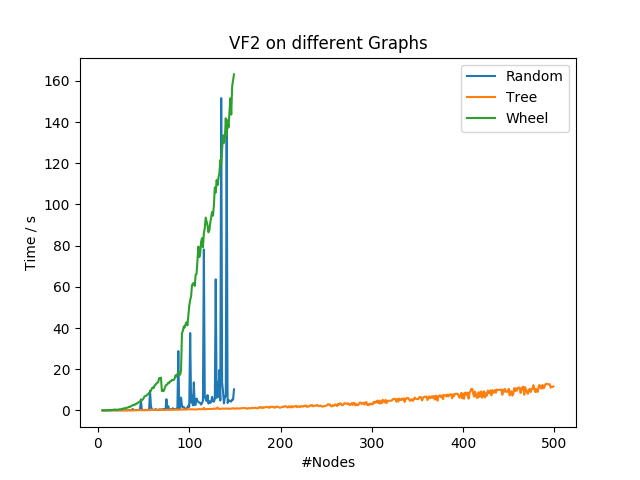
\includegraphics[scale=0.7]{vf2_all.png}
    \end{center}
    \caption{Elapsed time in function of alignment graphs' node set size. Representing random, tree and wheel graph alignments by VF2.}
\end{figure}

\begin{figure}
    \begin{center}
    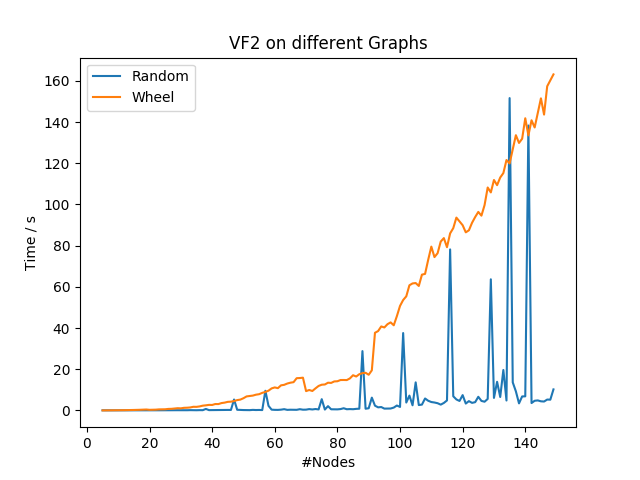
\includegraphics[scale=0.7]{vf2_all.wheel_random.png}
    \end{center}
    \caption{Elapsed time in function of alignment graphs' node set size. Representing random and wheel graph alignments by VF2.}
\end{figure}

\begin{figure}
    \begin{center}
    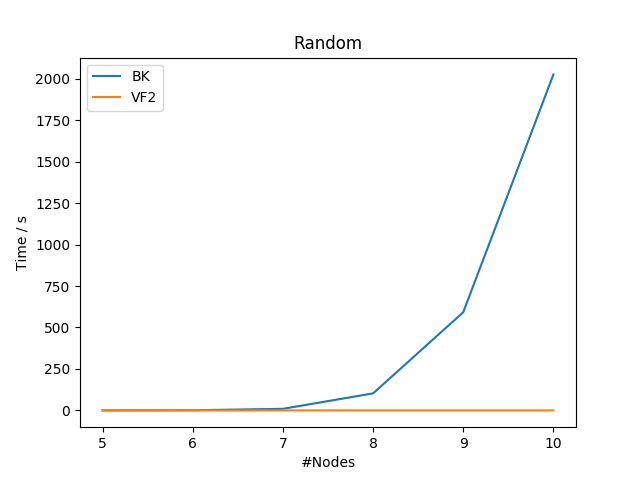
\includegraphics[scale=0.7]{vf2_bk_random.png}
    \end{center}
    \caption{Elapsed time in function of alignment graphs' node set size. Representing random graph alignments by VF2 and BK.}
\end{figure}

\begin{figure}
    \begin{center}
    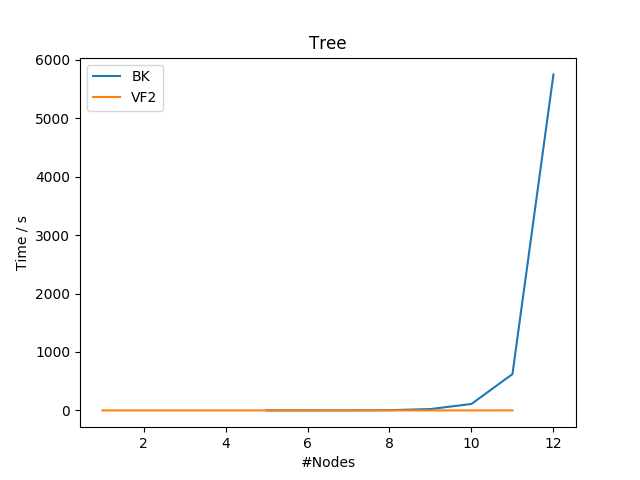
\includegraphics[scale=0.7]{vf2_bk_tree.png}
    \end{center}
    \caption{Elapsed time in function of alignment graphs' node set size. Representing tree graph alignments by VF2 and BK.}
\end{figure}

\begin{figure}
    \begin{center}
    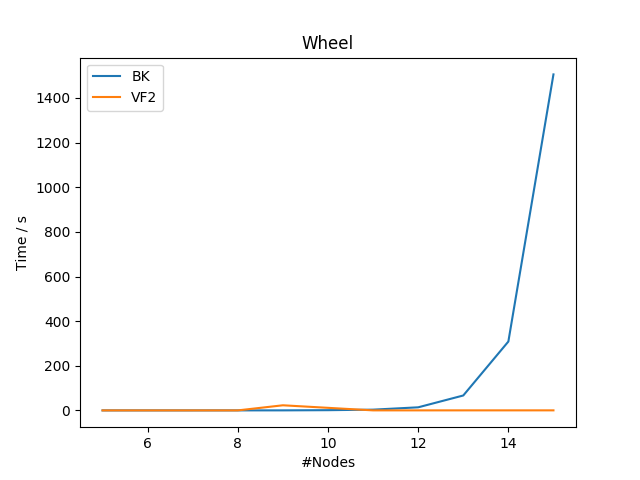
\includegraphics[scale=0.7]{vf2_bk_wheel.png}
    \end{center}
    \caption{Elapsed time in function of alignment graphs' node set size. Representing wheel graph alignments by VF2 and BK.}
\end{figure}


% ****************************************************************************
% BIBLIOGRAPHY AREA
% ****************************************************************************
\begin{footnotesize}
    \bibliography{multivitaminReadme}
    \bibliographystyle{unsrt}    
\end{footnotesize}
% ****************************************************************************
% END OF BIBLIOGRAPHY AREA
% ****************************************************************************

\end{document}





































